\vspace{10pt}

{\centering\subsection*{徐静蕾:端午节}}

\addcontentsline{toc}{subsection}{徐静蕾:端午节}

\renewcommand{\leftmark}{徐静蕾:端午节}

\begin{figure}[htbp]

\centering

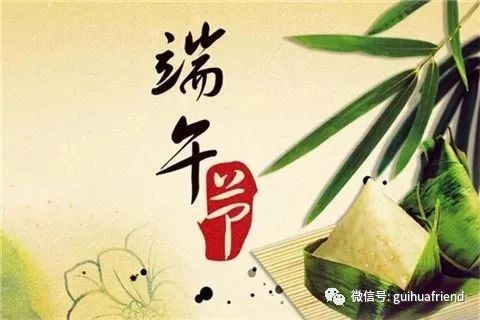
\includegraphics[width = .5\textwidth]{./ch/19.jpg}

\end{figure}





我国的传统节日有春节,元宵节,清明节,端午节,乞巧节,中秋节,重阳节,我最喜欢的是端午节。



端午节有很多的习俗,比如:赛龙舟、吃粽子、拜神祭祖、放纸鸢、挂五色丝线和佩戴香囊……

每年端午的时候我都会和妈妈一起包粽子,我们先去采粽叶,然后准备好糯米、葡萄干,红枣、白糖等各种各样的材料。

开始包粽子啦,我跟着妈妈先拿两片粽叶,再把粽叶弄成圆锥形,再把米放进去,放上两个葡萄干,然后用线扎紧。一个一个粽子就这么包好啦,一串一串的。

晚上我在睡觉的时候,妈妈还会给我讲有关于屈原的故事,每一年的端午节,我们都过得非常的开心!





\vspace{10pt}



作者:三(1)班 徐静蕾



指导老师:谢婷



投稿:2021年5月20日



发表:2021年5月21日






                



\vspace{10pt}

\hline



